%%%%%%%%%%%%%%%%%%%%%%%%%%%%%%%%%%%%%%%%%%%%%%%%%%%%%%%%%%%%%%%%%%%%%%%%%%%%%%%%
% IEEE Robotics and Automation Letters (RA-L) double-anonymous review manuscript
% Prepared with the official RAS/PaperCept ieeeconf class.
%%%%%%%%%%%%%%%%%%%%%%%%%%%%%%%%%%%%%%%%%%%%%%%%%%%%%%%%%%%%%%%%%%%%%%%%%%%%%%%%

\documentclass[letterpaper,10pt,conference]{ieeeconf}

\IEEEoverridecommandlockouts
\overrideIEEEmargins

% Explicitly keep the submitted PDF metadata anonymous.
\pdfinfo{
  /Title (Feature-Selection-Based Koopman Modeling and Robust LQR Control of Robots)
  /Author ()
  /Subject (Anonymous manuscript submitted for peer review)
  /Keywords (Koopman operator; basis function selection; data-driven modeling; LQR control; robust stability)
}

% Core packages required by the manuscript.
\usepackage{amsmath,amsfonts,amssymb}
\interdisplaylinepenalty=2500
\usepackage{mathtools}
\usepackage{algorithm}
\usepackage{algorithmic}
\usepackage{array}
\usepackage{textcomp}
\usepackage{url}
\usepackage{graphicx}
\usepackage{cite}
\usepackage{booktabs}
\usepackage{multirow}

% Algorithm labels.
\renewcommand{\algorithmicrequire}{\textbf{Input:}}
\renewcommand{\algorithmicensure}{\textbf{Output:}}

% Theorem environments.
\newtheorem{theorem}{Theorem}[section]
\newtheorem{proposition}{Proposition}[section]
\newtheorem{lemma}{Lemma}[section]
\newtheorem{definition}{Definition}[section]
\newtheorem{remark}{Remark}[section]
\newtheorem{assumption}{Assumption}[section]
\newtheorem{problem}{Problem}[section]

% Notation definitions.
\newcommand{\R}{\mathbb{R}}
\newcommand{\x}{\mathbf{x}}
\newcommand{\uvec}{\mathbf{u}}
\newcommand{\z}{\mathbf{z}}
\newcommand{\y}{\mathbf{y}}
\newcommand{\w}{\mathbf{w}}
\newcommand{\e}{\mathbf{e}}

% Bold matrices.
\newcommand{\Kmat}{\mathbf{K}}
\newcommand{\Dmat}{\mathbf{D}}
\newcommand{\A}{\mathbf{A}}
\newcommand{\B}{\mathbf{B}}
\newcommand{\C}{\mathbf{C}}
\newcommand{\I}{\mathbf{I}}
\newcommand{\Q}{\mathbf{Q}}
\newcommand{\Rmat}{\mathbf{R}}
\newcommand{\Zmat}{\mathbf{Z}}
\newcommand{\Umat}{\mathbf{U}}
\newcommand{\W}{\mathbf{W}}
\newcommand{\X}{\mathbf{X}}
\newcommand{\Y}{\mathbf{Y}}

% Feature-related notation.
\newcommand{\Phib}{\boldsymbol{\Phi}}
\newcommand{\XPhi}{\mathbf{X}_{\Phi}}
\newcommand{\YPhi}{\mathbf{Y}_{\Phi}}

% Operators.
\DeclareMathOperator{\tr}{tr}
\DeclareMathOperator{\rank}{rank}
\DeclareMathOperator{\diag}{diag}
\DeclareMathOperator*{\argmin}{arg\,min}

\hyphenation{op-tical net-works semi-conduc-tor IEEE-Xplore}

\title{\LARGE \bf
Feature-Selection-Based Koopman Modeling and Robust LQR Control of Robots
}


\author{\rule{0pt}{2.5ex}}

\begin{document}

\maketitle
\thispagestyle{empty}
\pagestyle{empty}

\begin{abstract}
Koopman operator theory with Extended Dynamic Mode Decomposition (EDMD) enables nonlinear dynamical systems to be represented by linear dynamics in a lifted space. However, the performance of EDMD strongly depends on the choice of basis functions: insufficient dictionaries limit approximation accuracy, whereas overcomplete dictionaries introduce redundancy, overfitting, and high computational cost. To address this issue, this paper proposes a feature-selection-based Koopman representation learning framework for robotic systems. A physics-informed overcomplete candidate library is first constructed, and a learnable feature selection matrix is then optimized to extract compact and informative linear combinations of candidate functions. The resulting modeling problem is formulated as a joint optimization over the Koopman matrices and the feature selection matrix, and a block coordinate descent algorithm is developed with convergence guarantees. Based on the learned lifted model, a feedforward-feedback Linear Quadratic Regulator controller is designed, where finite-dimensional approximation errors and external uncertainties are treated as bounded lumped disturbances. Lyapunov analysis proves that the closed-loop tracking error is ultimately uniformly bounded. Experiments on a three-degree-of-freedom robotic arm demonstrate improved modeling accuracy, tracking performance, and robustness.
\end{abstract}

\begin{keywords}
Koopman operator, basis function selection, data-driven modeling, LQR control, robust stability
\end{keywords}


% ================== Main Content ==================

\section{Introduction}
Modern robotic systems such as manipulators, mobile robots,
and soft robots exhibit highly nonlinear dynamics caused by mechanical
coupling, actuator characteristics, and uncertain interactions with the
environment~\cite{Brunton2022,DellaSantina2023}. Accurate dynamic models are
essential for high-performance control, but first-principles modeling becomes
difficult when the robot contains flexible structures, uncertain parameters, or
unmodeled interactions~\cite{Mamakoukas2021TRO}. Consequently,
data-driven models learned from operational data have become an important tool
for robotic prediction and control~\cite{Brunke2022,Tang2025survey,LiSu2026TCST,LiEtAl2026TCYB}.

Koopman operator theory offers a control-oriented way to
represent nonlinear dynamics by linear evolution in a lifted observable
space~\cite{Koopman1931,Korda2018conv}. Since the Koopman operator is
infinite-dimensional, practical methods rely on finite-dimensional
approximations. Extended Dynamic Mode Decomposition (EDMD) constructs such an
approximation by lifting the state through a user-specified dictionary of basis
functions~\cite{Williams2015EDMD,Korda2018conv}. The resulting lifted linear
models enable the use of linear-system tools, including Koopman-based model
predictive control and Koopman-based linear quadratic regulation, for nonlinear
robotic systems~\cite{Proctor2016DMDc,Korda2018MPC,Brunton2016Koopman}.

A key bottleneck of EDMD is the choice of basis functions.
In principle, the dictionary should span a subspace that is approximately
invariant under the Koopman operator. In practice, constructing such a
dictionary requires substantial prior knowledge of the underlying dynamics
\cite{Mauroy2019}. This leads to a tradeoff: a small dictionary may miss
important nonlinear features, whereas an overcomplete dictionary increases
computational cost, introduces redundancy and ill-conditioning, and may cause
overfitting~\cite{Mamakoukas2021TRO,ShiKarydis2022RAL}.

Existing studies mainly address this issue through learned dictionaries or
sparse selection. Deep learning methods can learn nonlinear coordinates from
data~\cite{Lusch2018,ShiMeng2022RAL,Ren2023TMech}, but the resulting features
are often difficult to interpret and analyze in robotic control. Sparse
regression methods select compact representations from large libraries
\cite{Li2017,Zhang2022Automatica}, but they may involve nonsmooth optimization
and sensitivity to noise and hyperparameters~\cite{WangEtAl2023RAL}. For robotic
systems, it is therefore desirable to retain the interpretability of
physics-informed candidate functions while avoiding the computational burden of
using the full overcomplete dictionary.

To this end, this paper proposes a Koopman representation learning framework
with a learnable feature selection mechanism. An overcomplete
physics-informed candidate library is first constructed, and an optimizable
selection matrix is then learned to extract compact linear combinations of the
candidate functions. Unlike PCA-based dimensionality reduction, which preserves
data variance, the proposed selection matrix is optimized directly for lifted
one-step prediction accuracy. The modeling problem is formulated as a joint
optimization over the Koopman matrices and the feature selection matrix, and a
block coordinate descent algorithm is developed with convergence guarantees.
Based on the learned lifted model, a feedforward-feedback Koopman-LQR
controller is designed for trajectory tracking. The finite-dimensional Koopman
approximation error is further treated as a bounded disturbance, which allows
the closed-loop tracking error to be analyzed through Lyapunov arguments.

The innovations and contributions of this paper are summarized as follows.
{\renewcommand{\labelenumi}{(\arabic{enumi})}
\begin{enumerate}
\item A feature-selection-based Koopman representation learning framework is
proposed for robotic systems. By constructing a physics-informed overcomplete
candidate function library and embedding a learnable feature selection matrix
into the lifted state, the proposed method extracts compact and informative
feature combinations while preserving the interpretability of the candidate
library.

\item The Koopman modeling task is formulated as a joint optimization problem
over the Koopman matrices and the feature selection matrix. The resulting
problem is solved by a block coordinate descent algorithm, where the matrix
update subproblems are explicitly characterized and convergence to a
stationary point is established under standard assumptions.

\item A robust feedforward-feedback Koopman-LQR controller is developed for
robotic trajectory tracking. By modeling finite-dimensional Koopman
approximation errors and external uncertainties as bounded lumped
disturbances, Lyapunov analysis proves that the closed-loop tracking error is
ultimately uniformly bounded and relates the disturbance level to the
steady-state tracking bound.
\end{enumerate}}

The rest of this paper is organized as follows. Section~\ref{sec:background}
introduces the preliminaries of Koopman operator theory and formulates the
problem considered in this paper. Section~\ref{sec:koopman} presents the
feature-selection-based Koopman representation learning framework and the
corresponding block coordinate descent algorithm. Section~\ref{sec:lqr}
develops the Koopman-based feedforward-feedback LQR controller and analyzes
the closed-loop robust tracking performance. Section~\ref{sec:experiments}
reports the experimental validation results on a real robotic platform.
Finally, Section~\ref{sec:conclusion} concludes this paper.

\textit{Notation:} Throughout this paper, unless otherwise stated,
$\|\cdot\|$ denotes the Euclidean norm for vectors and the induced $2$-norm
for matrices, $\|\cdot\|_1$ denotes the $\ell_1$ norm, and $\|\cdot\|_F$
denotes the Frobenius norm for matrices; $\mathbb{R}^n$ denotes the
$n$-dimensional Euclidean space; the superscripts $(\cdot)^\top$ and
$(\cdot)^\dagger$ denote the transpose and the Moore--Penrose pseudoinverse,
respectively; $\I_n$ denotes the $n \times n$ identity matrix;
$\mathbf{0}_{m \times n}$ denotes the $m \times n$ zero matrix;
$\tr(\cdot)$, $\rank(\cdot)$, and $\diag(\cdot)$ denote the trace, rank, and
diagonal matrix operator, respectively; $\mathcal{K}$ denotes the Koopman
operator; $\mathcal{H}$ denotes a Hilbert space; $\Phib(\x)$ denotes the
feature library; for a matrix $\mathbf{A}$, $\mathbf{A} \succeq 0$ and
$\mathbf{A} \succ 0$ mean that $\mathbf{A}$ is positive semidefinite and
positive definite, respectively.


% =========================================================
\section{Preliminaries and problem formulation}
\label{sec:background}
% =========================================================

\subsection{Koopman Operator Theory}
\label{subsec:koopman_theory}

Consider the discrete-time nonlinear system
\begin{equation}
\x_{k+1} = f(\x_k, \uvec_k),
\end{equation}
where $\x_k \in \R^n$ is the system state and $\uvec_k \in \R^m$ is the control input at time step $k$. The mapping $f: \R^n \times \R^m \to \R^n$ describes the state transition. It is assumed that $f$ is Lipschitz continuous on its domain.

Let \(\mathcal{H}\) be a Hilbert space of real-valued observation functions defined on the state space. For any observation function \(g \in \mathcal{H}\), when the control input is \(\uvec_k\), the discrete-time Koopman operator \(\mathcal{K}: \mathcal{H} \to \mathcal{H}\) is defined by the evolution of \(g\) along the system trajectories as
\begin{equation}
(\mathcal{K}g)(\x_k,\uvec_k) \triangleq g(f(\x_k,\uvec_k)) = g(\x_{k+1}).
\end{equation}

The core of Koopman operator theory is to lift the nonlinear dynamics
from the finite-dimensional state space to an infinite-dimensional
function space $\mathcal{H}$, thereby achieving linear evolution that
obeys the superposition principle:
\begin{equation}
\mathcal{K}(\alpha g_1 + \beta g_2) = \alpha \mathcal{K}g_1 + \beta \mathcal{K}g_2,
\end{equation}
where $g_1, g_2 \in \mathcal{H}$ are arbitrary observation functions and $\alpha, \beta \in \mathbb{R}$ are arbitrary
scalars. This linearity enables the application of linear-system tools to analyze
nonlinear dynamics after lifting.

\subsection{Problem Formulation}
\label{subsec:motivation}
As $\mathcal{H}$ is typically infinite-dimensional, EDMD approximates the Koopman operator in a finite-dimensional space spanned by a candidate function library $\{g_i\}_{i=1}^M$. The approximation quality depends critically on this library. A small library may miss essential nonlinear features, whereas an overcomplete library increases computational cost and may introduce redundancy and overfitting.

This accuracy--complexity tradeoff constitutes a central challenge in basis function selection for EDMD and related data-driven Koopman methods. To address this challenge and enable practical robotic control, this paper aims to: (1) learn a compact Koopman lifted representation from a physics-informed overcomplete candidate function library by using a feature selection matrix; and (2) design a robust feedforward-feedback LQR controller based on the learned lifted model to achieve reliable trajectory tracking under bounded lumped disturbances.


% =========================================================
\section{Koopman Representation Learning Based on Feature Selection Mechanism}
\label{sec:koopman}
% =========================================================

This section develops the feature-selection-based Koopman learning framework, including the joint optimization algorithm and the lumped-disturbance model used for robust control.

% ---------------------------------------------------------
\subsection{Learnable Feature Selection and Joint Optimization}
\label{subsec:algorithm}
% ---------------------------------------------------------
We first construct an overcomplete candidate observation function library $\Phib(\x):\R^n\to\R^P$, where $P\gg n$, to provide sufficient nonlinear expressiveness. To remove redundant components while preserving the physics-informed structure of the library, a learnable feature selection matrix $\Dmat\in\R^{N\times P}$ with $N\ll P$ is introduced. The resulting lifted coordinate is formally defined as follows.

{
\begin{definition}[Feature-selected augmented state]
Given the candidate library $\Phib(\x_k)$ and the selection matrix $\Dmat$, the compact feature vector and the augmented state are defined as
\begin{equation}
\boldsymbol{\eta}_k = \Dmat\Phib(\x_k), \qquad
\z_k = [\x_k^\top, \boldsymbol{\eta}_k^\top]^\top \in \R^{n+N}.
\end{equation}
Here, $\boldsymbol{\eta}_k$ preserves selected combinations of the overcomplete candidate functions, while the original physical state remains explicitly embedded in $\z_k$.
\end{definition}
}

Based on this augmented representation, we seek the following linear evolution model in the lifted space:
\begin{equation}
\label{eq:aug_dynamics}
\z_{k+1} = \A \z_k + \B \uvec_k,
\end{equation}
where $\A \in \R^{(n+N) \times (n+N)}$ is the Koopman matrix governing the linear dynamics in the lifted space, $\B \in \R^{(n+N) \times m}$ is the input matrix relating the control input to the augmented state evolution, and $\Kmat \in \R^{(n+N) \times (n+N+m)}$ is the augmented Koopman matrix defined as $\Kmat \triangleq [\A, \B]$.
This structure captures the nonlinear dynamics of the system through $\Dmat\Phib$, while simultaneously allowing lossless recovery of the physical state via the projection matrix $\C = [\I_n \ \mathbf{0}_{n \times N}]$ according to
\begin{equation}
\x_k = \C\z_k,
\end{equation}
which facilitates the subsequent full-state feedback design.
Figure~\ref{fig:koopman_framework} illustrates the proposed Koopman representation learning framework.
\begin{figure*}[!t]
\centering
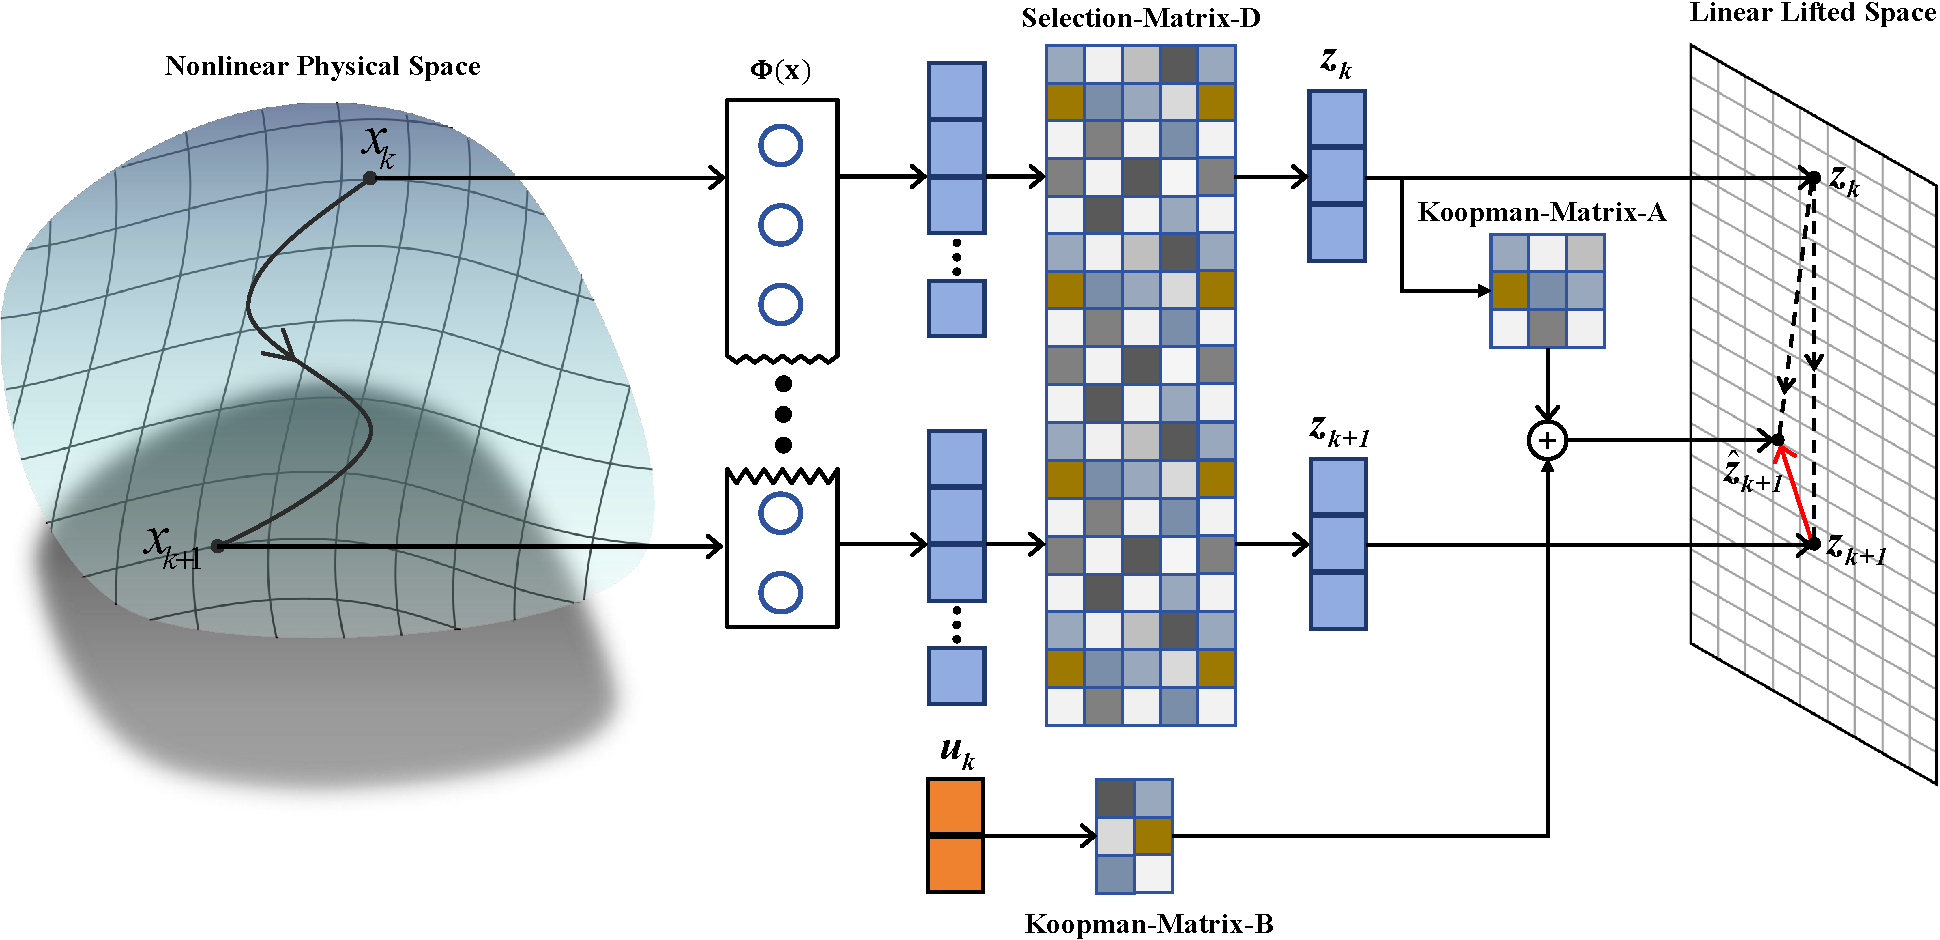
\includegraphics[width=0.85\textwidth]{pictures/koopman_framework.pdf}
\caption{Koopman representation learning with the learnable feature selection mechanism.}
\label{fig:koopman_framework}
\end{figure*}

Given a trajectory dataset $\{\x_k, \uvec_k\}_{k=1}^{T+1}$, where $\x_k \in \R^n$ represents the robot state (e.g., joint positions and velocities) and $\uvec_k \in \R^m$ denotes the control torque applied to each joint, which yields $T$ one-step transition pairs, we construct the state snapshot matrices $\X = [\x_1, \dots, \x_T]$ and $\Y = [\x_2, \dots, \x_{T+1}]$, the input matrix $\Umat = [\uvec_1, \dots, \uvec_T]$, and the feature matrices $\XPhi = [\Phib(\x_1), \dots, \Phib(\x_T)]$ and $\YPhi = [\Phib(\x_2), \dots, \Phib(\x_{T+1})]$. For a given $\Dmat$, the lifted state data matrices are defined as
\begin{equation}
\Zmat(\Dmat) =
\begin{bmatrix}
\X \\ \Dmat \XPhi
\end{bmatrix}, \qquad
\Zmat^+(\Dmat) =
\begin{bmatrix}
\Y \\ \Dmat \YPhi
\end{bmatrix}.
\end{equation}
We formulate the joint optimization problem as
\begin{equation}
\label{eq:objective}
\begin{aligned}
L(\Kmat,\Dmat) &= \frac{1}{2}
\left\|
\Zmat^+(\Dmat) - \Kmat
\begin{bmatrix}
\Zmat(\Dmat) \\ \Umat
\end{bmatrix}
\right\|_F^2 \\
&\quad + \lambda\|\Dmat\|_1 + \beta\|\Kmat\|_F^2, \\
(\Kmat^\star, \Dmat^\star) &= \arg\min_{\Kmat,\Dmat} \; L(\Kmat,\Dmat).
\end{aligned}
\end{equation}
where $\lambda>0$ and $\beta>0$ are the regularization coefficients. The $\ell_1$ regularization on $\Dmat$ promotes sparse linear combinations of informative candidate functions from the overcomplete candidate function library. Meanwhile, the objective function enforces accurate one-step prediction of both the physical state and the projected feature components in the lifted state, thereby discouraging trivial solutions for $\Dmat$. When $\Dmat = \I_P$ and the regularization terms $\lambda\|\Dmat\|_1$ and $\beta\|\Kmat\|_F^2$ are removed, the formulation reduces to standard EDMD.

Since the optimization problem in~\eqref{eq:objective} is nonconvex in
the joint variables $(\Kmat,\Dmat)$, we adopt a two-block coordinate
descent (BCD) algorithm~\cite{Tseng2001} to solve it by alternately
updating the two variable blocks. Let $(\Kmat^{(t)},\Dmat^{(t)})$
denote the iterates at iteration $t$, and define the corresponding objective value as
\[
L^{(t)} := L(\Kmat^{(t)},\Dmat^{(t)}).
\]
At each iteration, the two variable blocks are updated alternately by solving a strongly convex $\Kmat$-subproblem and a convex $\Dmat$-subproblem.

\textit{1) $\Kmat$-subproblem:}
With $\Dmat^{(t)}$ fixed, define
\[
\mathbf{Y}_{\mathrm{aug}}^{(t)} := \Zmat^+(\Dmat^{(t)}), \qquad
\W^{(t)} :=
\begin{bmatrix}
\Zmat(\Dmat^{(t)}) \\ \Umat
\end{bmatrix}.
\]
Then, the $\Kmat$-subproblem is given by
\[
\min_{\Kmat} \; 
\frac{1}{2}\|\mathbf{Y}_{\mathrm{aug}}^{(t)}
- \Kmat \W^{(t)}\|_F^2
+ \beta\|\Kmat\|_F^2 .
\]
This is a standard ridge regression problem. Setting the gradient with respect to $\Kmat$ to zero gives
\[
-(\mathbf{Y}_{\mathrm{aug}}^{(t)} - \Kmat \W^{(t)})
\W^{(t)\top} + 2\beta\Kmat = \mathbf{0},
\]
from which the closed-form update is derived as
\begin{equation}
\label{eq:K_update}
\Kmat^{(t+1)}
= \Zmat^+(\Dmat^{(t)}) \W^{(t)\top}
\bigl( \W^{(t)} \W^{(t)\top} + 2\beta \I \bigr)^{-1}.
\end{equation}

For the $\Kmat$ update, the ridge regularization makes the subproblem strongly convex for any fixed $\Dmat^{(t)}$ and $\beta>0$, so the minimizer in~\eqref{eq:K_update} is unique.

\textit{2) $\Dmat$-subproblem:} With $\Kmat^{(t+1)}$ fixed, the $\Dmat$-subproblem is formulated as
\begin{equation}
\label{eq:D_subproblem}
\Dmat^{(t+1)} = \arg\min_{\Dmat} \; J^{(t)}(\Dmat),
\end{equation}
where
\begin{equation}
\label{eq:D_objective}
J^{(t)}(\Dmat) = \frac{1}{2}\left\| \Zmat^+(\Dmat) - \Kmat^{(t+1)}
\begin{bmatrix}
\Zmat(\Dmat) \\ \Umat
\end{bmatrix} \right\|_F^2
+ \lambda\|\Dmat\|_1.
\end{equation}
To see this, we write $\Kmat^{(t+1)} = [\A^{(t+1)},\B^{(t+1)}]$ and partition $\A^{(t+1)}$ according to the augmented state structure. Since both $\Zmat(\Dmat)$ and $\Zmat^+(\Dmat)$ depend affinely on $\Dmat$, the residual
\[
\Zmat^+(\Dmat) - \Kmat^{(t+1)}
\begin{bmatrix}
\Zmat(\Dmat) \\ \Umat
\end{bmatrix}
\]
is affine in $\Dmat$. Hence, the data-fitting term in~\eqref{eq:D_objective} is a convex quadratic function of $\Dmat$, and the subproblem can be efficiently solved using proximal gradient methods~\cite{Beck2009ISTA}.

For the $\Dmat$ update, the subproblem in~\eqref{eq:D_subproblem} is a convex composite optimization problem consisting of a quadratic data-fitting term and a separable $\ell_1$ regularizer. Hence, it can be solved by standard proximal gradient updates.

Let $T_{\max}$ denote the maximum number of iterations and let $\varepsilon>0$ denote the convergence tolerance. The above block structure leads to the BCD procedure summarized in Algorithm~\ref{alg:altmin}. Its convergence property is stated as follows.

\begin{theorem}[Convergence of the BCD Algorithm]
\label{thm:altmin_convergence}
Suppose that $\lambda>0$ and $\beta>0$, and that each subproblem is solved to optimality at every iteration. Then the sequence $\{(\Kmat^{(t)}, \Dmat^{(t)})\}$ generated by Algorithm~\ref{alg:altmin} satisfies:
\begin{enumerate}
\item The objective values $L^{(t)}$ are monotonically nonincreasing and converge to a finite limit;
\item The iterates $\{(\Kmat^{(t)},\Dmat^{(t)})\}$ remain bounded;
\item Every accumulation point of the sequence is a first-order stationary point of~\eqref{eq:objective}.
\end{enumerate}
\end{theorem}

\begin{proof}
First, since each block is minimized exactly while the other block is fixed, the two successive updates in Algorithm~\ref{alg:altmin} yield
\[
\begin{aligned}
L(\Kmat^{(t+1)},\Dmat^{(t)}) &\le L(\Kmat^{(t)},\Dmat^{(t)}), \\
L(\Kmat^{(t+1)},\Dmat^{(t+1)}) &\le L(\Kmat^{(t+1)},\Dmat^{(t)}).
\end{aligned}
\]
Therefore, $L^{(t+1)} \le L^{(t)}$, and the objective sequence is monotonically nonincreasing. Since $L(\Kmat,\Dmat) \ge 0$, it converges to a finite limit.

Second, from $L^{(t)} \le L^{(0)}$ and the nonnegativity of the data-fitting term, we obtain
\[
\beta\|\Kmat^{(t)}\|_F^2 + \lambda\|\Dmat^{(t)}\|_1 \le L^{(0)}.
\]
Hence, the sequence $\{\Kmat^{(t)}\}$ is bounded. The sequence $\{\Dmat^{(t)}\}$ is also bounded, because boundedness in the $\ell_1$ norm implies boundedness in the Frobenius norm for finite-dimensional matrices.

Finally, the objective in~\eqref{eq:objective} is the sum of a continuously differentiable data-fitting term and a convex separable nonsmooth regularization term, and each block subproblem is solved to optimality at every iteration. By the standard convergence results for block coordinate descent applied to nonsmooth objectives~\cite{Tseng2001}, every accumulation point of $\{(\Kmat^{(t)},\Dmat^{(t)})\}$ is a first-order stationary point of~\eqref{eq:objective}.
\end{proof}

\begin{algorithm}[htbp]
\caption{Block Coordinate Descent Algorithm for Koopman Representation Learning}
\label{alg:altmin}
\begin{algorithmic}[1]
\REQUIRE Data $(\X,\Y,\Umat)$, basis library $\Phib$, parameters $\lambda,\beta$, initialization $\Dmat^{(0)}$
\ENSURE Learned $\Kmat^\star$ and $\Dmat^\star$
\FOR{$t = 0, 1, \dots, T_{\max}-1$}
    \STATE Update $\Kmat^{(t+1)}$ using~\eqref{eq:K_update}
    \STATE Update $\Dmat^{(t+1)}$ by solving~\eqref{eq:D_subproblem} via a proximal gradient method
    \IF{$|L^{(t+1)} - L^{(t)}| < \varepsilon$}
        \STATE \textbf{break}
    \ENDIF
\ENDFOR
\end{algorithmic}
\end{algorithm}

% ---------------------------------------------------------
\subsection{Lumped Disturbance Analysis}
\label{subsec:error_quantification}
% ---------------------------------------------------------

The learned Koopman model captures the dominant system dynamics, but the finite-dimensional lifted model inevitably contains approximation residuals. In addition, sensor noise and environmental disturbances may appear during robot operation. We collect these effects into a lumped disturbance term $\w_k$, and the actual evolution in the lifted space is written as
\begin{equation}
\label{eq:lumped_model}
\z_{k+1} = \A\z_k + \B\uvec_k + \w_k,
\end{equation}
where $\A$ and $\B$ are the learned Koopman state-transition matrix and input matrix, respectively, obtained from Algorithm~\ref{alg:altmin}.

When the state and input are constrained to compact sets, the Koopman approximation error is theoretically bounded~\cite{Korda2018MPC}. Sensor noise and environmental disturbances are also bounded in practical robotic systems due to hardware limits and operating conditions. This motivates the following assumption.

{
\begin{assumption}[Bounded lumped disturbance]
\label{assump:bounded_disturbance}
There exists a constant $\delta_w>0$ such that the lumped disturbance in~\eqref{eq:lumped_model} satisfies
\begin{equation}
\|\w_k\| \le \delta_w, \quad \forall k.
\end{equation}
\end{assumption}
}

Assumption~\ref{assump:bounded_disturbance} provides the interface between the learned finite-dimensional Koopman model and the robust tracking analysis. A smaller approximation residual corresponds to a smaller admissible disturbance level, which is reflected in the ultimate tracking bound derived in Section~\ref{subsec:lqr_robust}.


% =========================================================
\section{LQR Control Based on Koopman Model}
\label{sec:lqr}
% =========================================================

This section designs a feedforward-feedback Koopman-LQR controller for the disturbed lifted model~\eqref{eq:lumped_model} and establishes the ultimate boundedness of the closed-loop tracking error.

\subsection{Feedforward-Feedback Robust Controller Design}
\label{subsec:lqr_design}

To achieve robust trajectory tracking, we design the controller based on the disturbed augmented linear model~\eqref{eq:lumped_model} obtained from the learned Koopman model in Section~\ref{sec:koopman}.
First, let $\{\x_k^{\text{ref}}\}_{k=0}^{\infty}$ denote the desired reference trajectory in the physical state space. By lifting this trajectory through the feature mapping and the learned selection matrix $\Dmat^\star$, we obtain the corresponding lifted reference trajectory: 
\begin{equation}
\z_k^{\text{ref}} = [{\x_k^{\text{ref}}}^\top, {(\Dmat^\star\Phib(\x_k^{\text{ref}}))}^\top]^\top.
\end{equation}

To balance the tracking accuracy and the control efforts, we define the following infinite-horizon quadratic cost function:
\begin{equation}
\label{eq:lqr_cost}
J = \sum_{k=0}^{\infty} \left( (\z_k - \z_k^{\text{ref}})^\top \Q (\z_k - \z_k^{\text{ref}}) + \uvec_k^\top \Rmat \uvec_k \right),
\end{equation}
where $\Q = \C^\top \Q_x \C \succeq 0$ is the lifted-state weight matrix, $\Q_x$ is the weight matrix in the original state space, and $\Rmat \succ 0$ is the control input weight matrix.

Assume that the physical system is controllable and that the training data are sufficiently informative such that the learned linear model $(\A,\B)$ is stabilizable. Under these conditions, the standard LQR theory yields a unique optimal state-feedback gain $\Kmat_{\text{lqr}}$, which renders the closed-loop matrix $\A_{\text{cl}} = \A - \B\Kmat_{\text{lqr}}$ Schur stable.

To guarantee the trajectory tracking of the robots, we propose the following composite feedforward-feedback control law:
\begin{equation}
\label{eq:lqr_total}
\uvec_k = \uvec_k^{\mathrm{ff}} - \Kmat_{\text{lqr}}(\z_k - \z_k^{\text{ref}}).
\end{equation}
The feedforward term $\uvec_k^{\mathrm{ff}}$ is used to compensate for the known dynamics along the reference trajectory and is computed as
\begin{equation}
\label{eq:uff}
\uvec_k^{\mathrm{ff}} = \B^{\dagger}(\z_{k+1}^{\text{ref}} - \A\z_k^{\text{ref}}),
\end{equation}
where $\B^{\dagger}$ denotes the Moore-Penrose pseudoinverse of $\B$. Figure~\ref{fig:controller} illustrates the structure of the proposed Koopman-LQR controller.

\begin{figure}[!t]
\centering
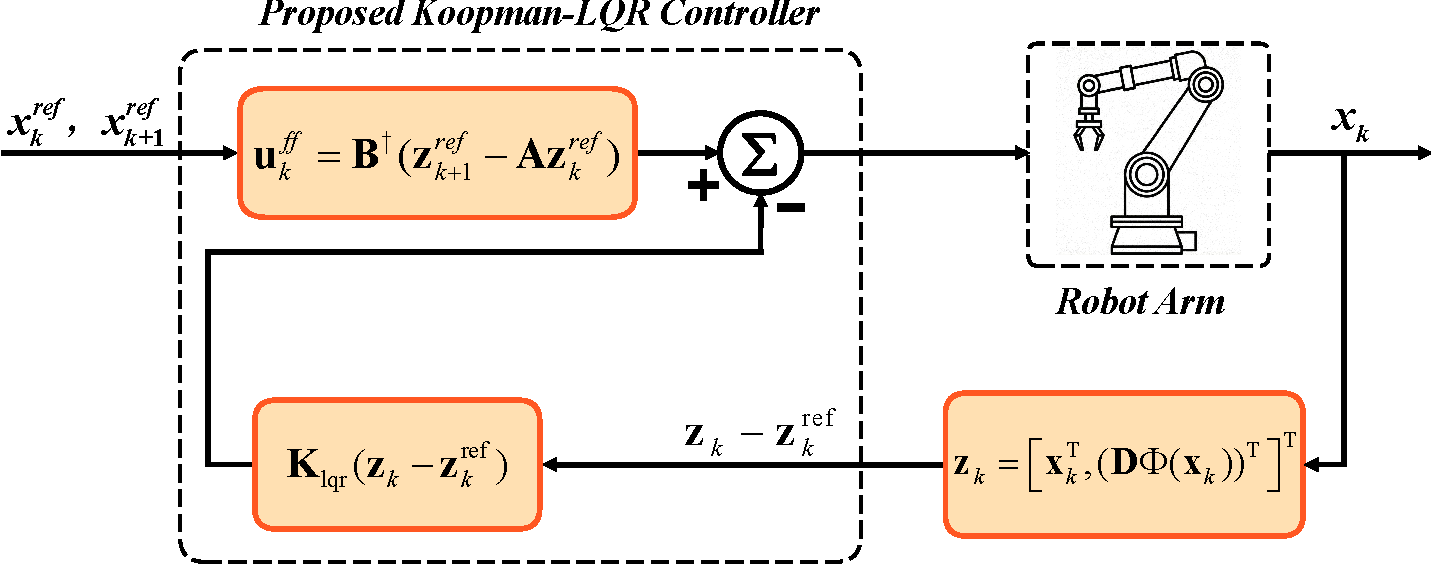
\includegraphics[width=0.48\textwidth]{pictures/controller.pdf}
\caption{The proposed Koopman-based feedforward-feedback LQR control structure.}
\label{fig:controller}
\end{figure}


\subsection{Stability Analysis}
\label{subsec:lqr_robust}

Based on the feedforward-feedback controller~\eqref{eq:lqr_total}, we present the following stability result.

The key observation is that the feedforward term removes the nominal reference dynamics, whereas the LQR feedback stabilizes the deviation around the lifted reference trajectory. Therefore, the closed-loop tracking error can be analyzed as a stable linear system driven by the lumped disturbance.

\begin{theorem}[Robust Tracking Performance]
\label{thm:lqr_uub}
Consider the system~\eqref{eq:lumped_model} under the control law~\eqref{eq:lqr_total}. Suppose that Assumption~\ref{assump:bounded_disturbance} holds. Then the closed-loop system achieves ultimately uniformly bounded (UUB) tracking, i.e., there exists $R > 0$ such that, for any initial condition, there exists a finite time $K$ for which $\|\e_k\| \le R$ for all $k \ge K$.
\end{theorem}

\begin{proof}
Define the tracking error as $\e_k := \z_k - \z_k^{\text{ref}}$. Substituting the control law~\eqref{eq:lqr_total} into the disturbed augmented model~\eqref{eq:lumped_model}, and using the definition of the feedforward term in~\eqref{eq:uff}, the closed-loop error dynamics are given by
\begin{equation}
\label{eq:error_dynamics}
\e_{k+1} = (\A - \B\Kmat_{\text{lqr}})\e_k + \w_k = \A_{\text{cl}}\e_k + \w_k,
\end{equation}
where $\A_{\text{cl}} := \A - \B\Kmat_{\text{lqr}}$ denotes the closed-loop system matrix. By the stabilizability assumption in Section~\ref{subsec:lqr_design} and the standard LQR theory, $\A_{\text{cl}}$ is Schur stable. Hence, there exist positive definite matrices $\mathbf{P} \succ 0$ and $\mathbf{S} \succ 0$ satisfying the discrete-time Lyapunov equation
\[
\A_{\text{cl}}^\top \mathbf{P} \A_{\text{cl}} - \mathbf{P} = -\mathbf{S}.
\]
Consider the Lyapunov function $V_k = \e_k^\top \mathbf{P} \e_k$. Then, along the trajectories of~\eqref{eq:error_dynamics},
\begin{align}
\Delta V_k &= V_{k+1} - V_k \nonumber \\
&= \e_k^\top (\A_{\text{cl}}^\top \mathbf{P} \A_{\text{cl}} - \mathbf{P}) \e_k
+ 2\e_k^\top \A_{\text{cl}}^\top \mathbf{P}\w_k
+ \w_k^\top \mathbf{P}\w_k \nonumber \\
&= -\e_k^\top \mathbf{S} \e_k
+ 2\e_k^\top \A_{\text{cl}}^\top \mathbf{P}\w_k
+ \w_k^\top \mathbf{P}\w_k,
\end{align}
where the last equality follows from the discrete-time Lyapunov equation. By the boundedness of $\w_k$ and the Cauchy--Schwarz inequality, it follows that when $\|\e_k\|$ exceeds a threshold $R$ determined by $\delta_w$, one has $\Delta V_k < 0$. Therefore, the error trajectory enters and remains within the bounded set $\mathcal{B}_R = \{\e : \|\e\| \le R\}$~\cite{Blanchini2008,Khalil2002}.
\end{proof}

Since the projection matrix $\C$ satisfies $\|\C\| = 1$, the error bound in the lifted space directly guarantees the tracking accuracy in the original state space:
\[
\|\x_k - \x_k^{\text{ref}}\| = \|\C\e_k\| \le \|\e_k\| \le R.
\]
Furthermore, the steady-state error bound can be upper bounded by a linear function of the disturbance level, i.e.,
\[
R \le c\,\delta_w,
\]
where the constant $c > 0$ depends only on the spectral properties of the closed-loop matrix $\A_{\text{cl}}$~\cite{Blanchini2008}. This relationship connects the Koopman modeling accuracy with the closed-loop performance: reducing the approximation component of $\w_k$ decreases $\delta_w$ and hence shrinks the ultimate tracking bound.



% =========================================================
\section{Experimental Validations}
\label{sec:experiments}
% =========================================================


% ---------------------------------------------------------
\subsection{Experimental Platform and Data Collection}
\label{subsec:exp_setup}
% ---------------------------------------------------------

Experiments were conducted on a Geomagic Touch\textsuperscript{\textregistered} robot arm, whose mechanical structure is shown in Fig.~\ref{fig:geomagic_touch}. The device has three revolute joints with integrated encoders for real-time measurement of joint position and velocity. The force-feedback stylus at the end-effector was kept fixed during the experiments so that the joint-space dynamics could be isolated.

According to the technical specifications provided by the manufacturer, the motion ranges of joints 1, 2, and 3 are $[-1.3, 0.66]$ rad, $[0.2, 2.0]$ rad, and $[-0.65, 0.87]$ rad, respectively. Joints 2 and 3 are mechanically coupled, so the allowable range of joint 3 is affected when joint 2 approaches its motion limit. To reduce the influence of this coupling, the data collection experiments were conducted to avoid the coupled boundary as much as possible.

During the data collection experiments, continuous random control torques were applied to the three joints to excite the system dynamics. The sampling period was 0.004 s. In total, 20 trajectories were collected, each with a duration of 20 s, containing joint positions, velocities, and the corresponding control inputs. The complete dataset was split into training, validation, and test sets with a ratio of 15:4:1.

\begin{figure}[htbp]
\centering
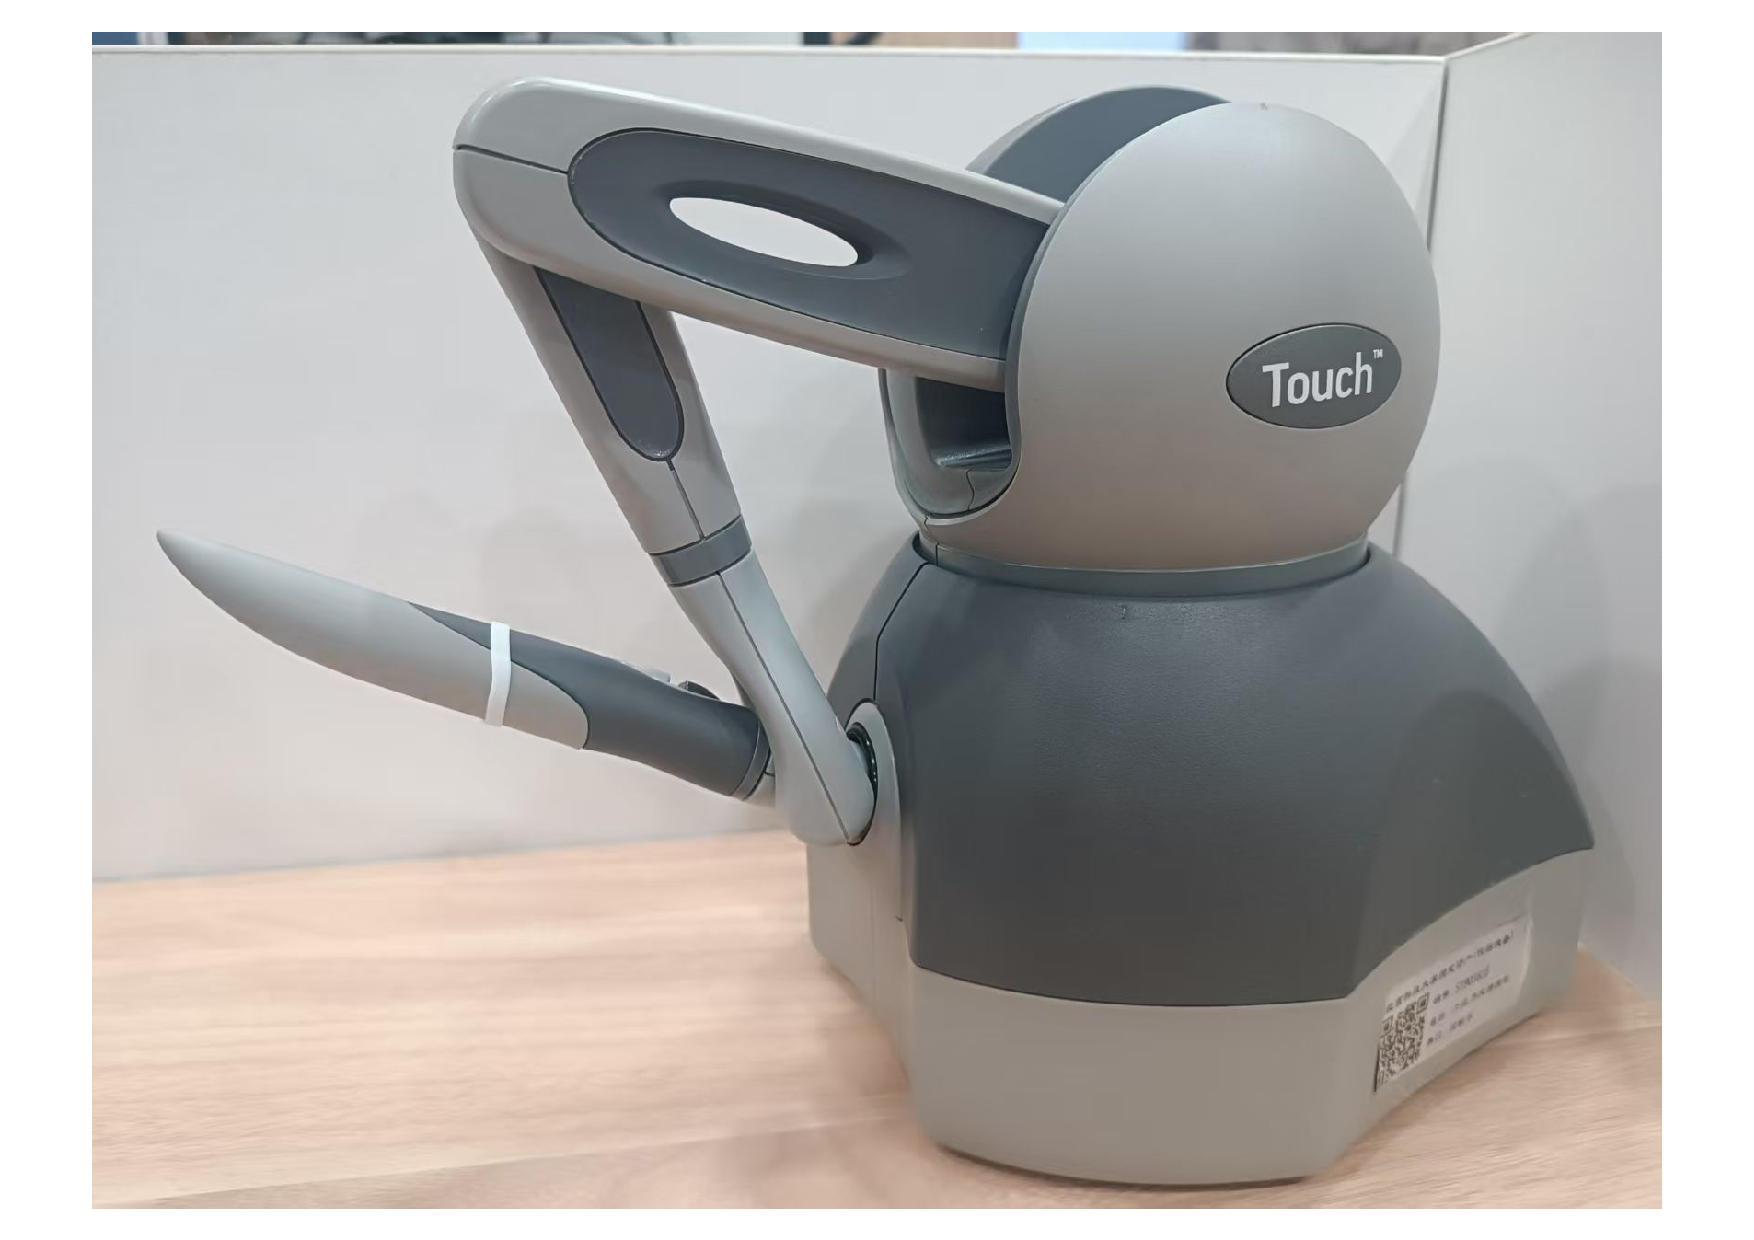
\includegraphics[width=0.75\columnwidth]{pictures/geomagic_touch.pdf}
\caption{The Geomagic Touch robot arm.}
\label{fig:geomagic_touch}
\end{figure}

% ---------------------------------------------------------
\subsection{Model Prediction Accuracy Comparison}
\label{subsec:modeling_accuracy}
% ---------------------------------------------------------

For comparison, two Koopman baselines were used: EDMDDL~\cite{Li2017}, which learns a 60-dimensional dictionary using a five-layer neural network with 512 ReLU neurons per layer, and standard EDMD~\cite{Williams2015EDMD}, which directly uses the full 364-dimensional candidate function library. FS-EDMD uses the same candidate function library as standard EDMD but learns a compact selection matrix $\Dmat \in \R^{60 \times 364}$. All methods were trained on the same training set and evaluated by an 800-step continuous rollout prediction on an independent test trajectory.

Fig.~\ref{fig:position_comparison} shows the joint position prediction results. FS-EDMD maintains the closest agreement with the measured trajectory over the 3.2~s prediction horizon, whereas EDMDDL gradually drifts and standard EDMD accumulates larger errors. The full-state prediction errors, including both joint positions and velocities, are summarized in Table~\ref{tab:modeling_accuracy}.

\begin{figure}[htbp]
\centering

\includegraphics[width=0.4\textwidth]{pictures/position_comparison.png}
\caption{Comparison of the joint position prediction results obtained by FS-EDMD, EDMDDL, and the standard EDMD.}
\label{fig:position_comparison}
\end{figure}

As shown in Table~\ref{tab:modeling_accuracy}, FS-EDMD achieves the lowest full-state prediction errors, with MSE, RMSE, and MAE of 0.3520, 0.5933, and 0.3202, respectively. These correspond to reductions of 40.7\%, 23.0\%, and 29.6\% over EDMDDL, and 51.5\%, 30.3\%, and 36.2\% over standard EDMD.

\begin{table}[htbp]
\centering
\caption{Modeling Accuracy Comparison of the Three Methods}
\label{tab:modeling_accuracy}
\begin{tabular}{lccc}
\toprule
Method & MSE & RMSE & MAE \\
\midrule
FS-EDMD & \textbf{0.3520} & \textbf{0.5933} & \textbf{0.3202} \\
EDMDDL & 0.5936 & 0.7704 & 0.4550 \\
Standard EDMD & 0.7256 & 0.8518 & 0.5022 \\
\bottomrule
\end{tabular}
\end{table}

\footnotetext[1]{\label{fn:pred_metrics}
$\mathrm{MSE} = \frac{1}{T}\sum_{k=1}^{T}\|\x_k - \hat{\x}_k\|^2$,
$\mathrm{RMSE} = \sqrt{\mathrm{MSE}}$,
$\mathrm{MAE} = \frac{1}{T}\sum_{k=1}^{T}\|\x_k - \hat{\x}_k\|$,
where $\hat{\x}_k$ denotes the predicted state at time step $k$.}


% ---------------------------------------------------------
\subsection{Trajectory Tracking Control Performance Evaluation}
\label{subsec:control_performance}
% ---------------------------------------------------------

Trajectory tracking experiments were conducted in the joint space using sinusoidal and irregular references. The Koopman-LQR controller was implemented with the FS-EDMD model and the feedforward-feedback structure in Section~\ref{sec:lqr}. The weighting matrices were set to $\Q=\diag(100,10,100,10,100,10)$ and $\Rmat=\I_3$, and a PID controller with empirically tuned gains $K_p=25$, $K_i=0.1$, and $K_d=2.5$ was used as the baseline.

For sinusoidal tracking, the reference trajectories for the three joints
were defined as
\begin{equation}
    q_i^{\text{ref}}(t) = A_i \sin(\omega_i t) + b_i, \quad i = 1, 2, 3,
\end{equation}
where $q_i^{\text{ref}}$ denotes the desired joint position. The amplitudes were set to $A_1=0.5$~rad, $A_2=0.4$~rad, and $A_3=0.35$~rad, with $f_i=0.25$~Hz and $b_i=0$ for all joints. As shown in Fig.~\ref{fig:control_comparison_sinusoidal}, Koopman-LQR tracks the references more accurately than PID, especially on joints 2 and 3.

\begin{figure}[htbp]
\centering
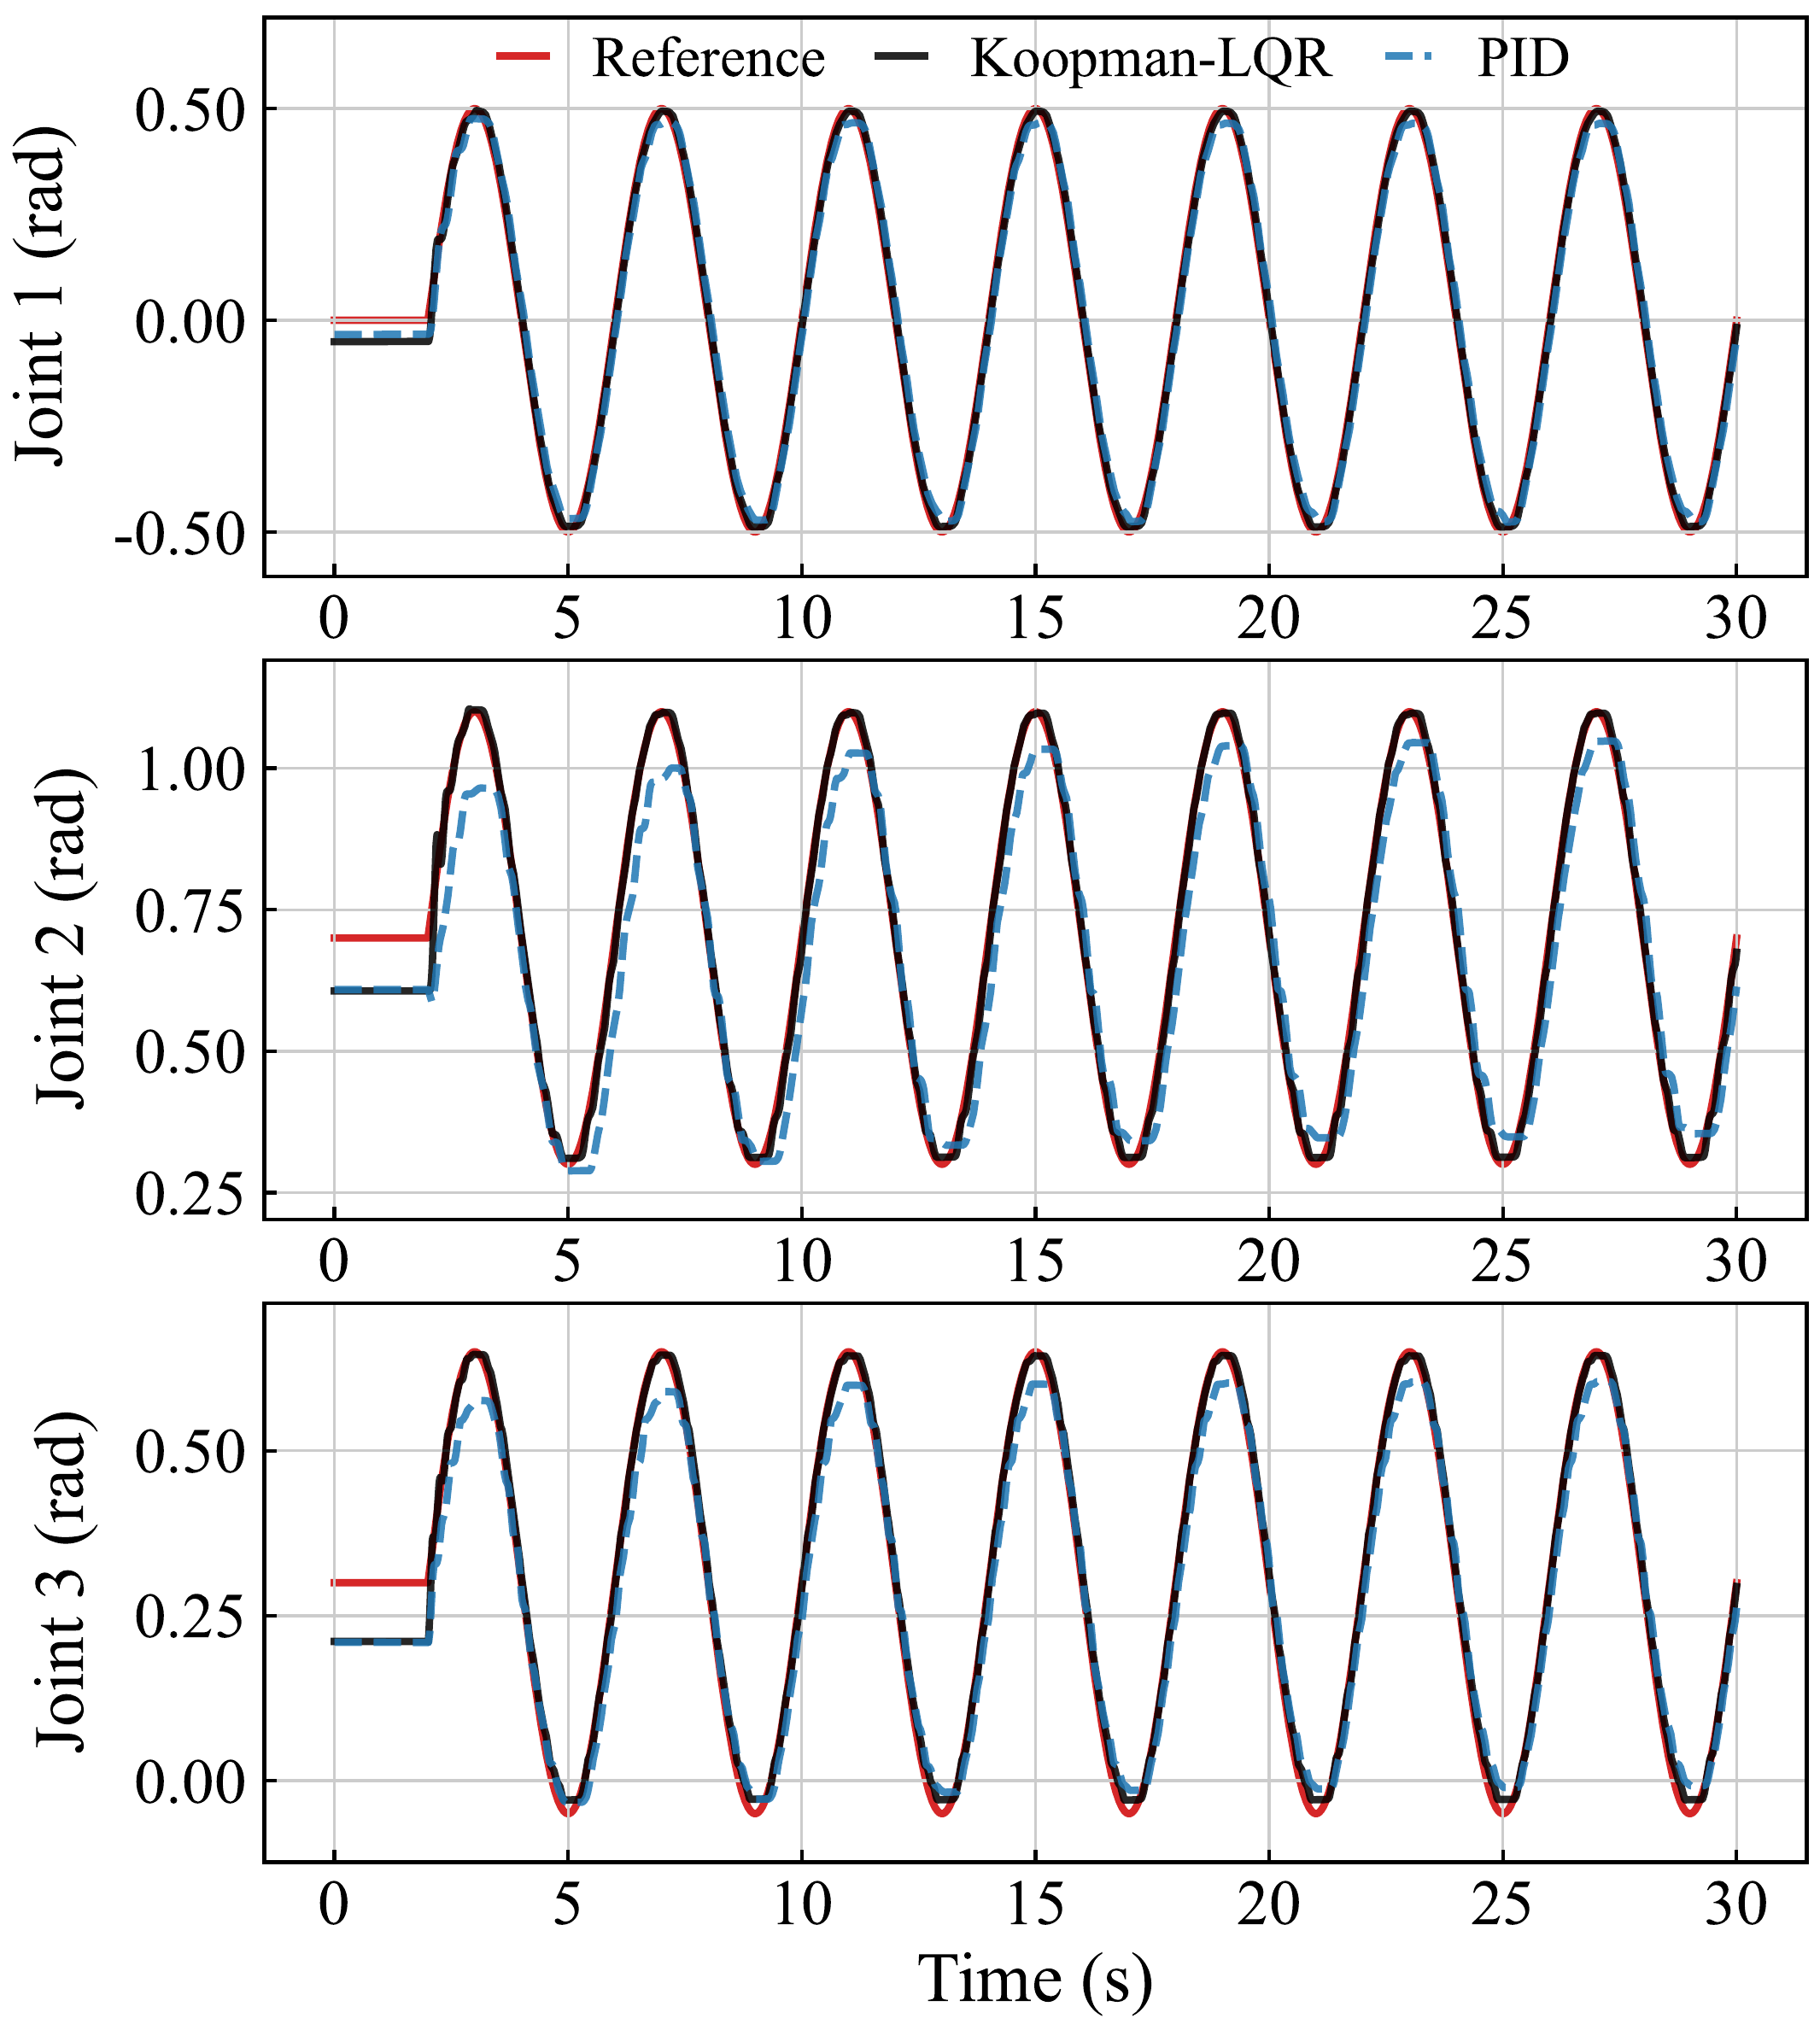
\includegraphics[width=0.4\textwidth]{pictures/control_comparison_sinusoidal.png}
\caption{Comparison of the sinusoidal trajectory tracking performance of the Koopman-LQR and the PID Controllers.}
\label{fig:control_comparison_sinusoidal}
\end{figure}

For irregular tracking, joints 1 and 2 used composite references formed by the superposition of three sinusoidal components:
\begin{equation}
q_j^{\text{ref}}(t) = \sum_{l=1}^{3} A_{j,l} \sin(2\pi f_{j,l} t + \phi_{j,l}),
\quad j = 1, 2,
\end{equation}
where $A_{j,l}$, $f_{j,l}$, and $\phi_{j,l}$ denote the amplitude, frequency, and phase of the $l$-th component, respectively. The parameters are listed in Table~\ref{tab:irregular_params}. Due to the mechanical coupling between joints 2 and 3, joint 3 used $q_3^{\text{ref}}(t)=0.35\sin(2\pi\cdot0.25t)$.

\begin{table}[htbp]
\centering
\caption{Irregular Reference Parameters}
\label{tab:irregular_params}
\small
\setlength{\tabcolsep}{3.5pt}
\begin{tabular}{ccccc}
\toprule
Joint & $l$ & $A_{j,l}$ (rad) & $f_{j,l}$ (Hz) & $\phi_{j,l}$ (rad) \\
\midrule
\multirow{3}{*}{1} & 1 & 0.25 & 0.15 & $0$ \\
                   & 2 & 0.15 & 0.40 & $\pi/4$ \\
                   & 3 & 0.08 & 0.80 & $\pi/3$ \\
\midrule
\multirow{3}{*}{2} & 1 & 0.22 & 0.18 & $\pi/6$ \\
                   & 2 & 0.12 & 0.45 & $0$ \\
                   & 3 & 0.06 & 0.90 & $\pi/2$ \\
\bottomrule
\end{tabular}
\end{table}

The tracking results are shown in Fig.~\ref{fig:control_comparison_irregular}. Koopman-LQR follows the composite reference more accurately during fast transitions, whereas PID produces larger tracking errors.

\begin{figure}[htbp]
\centering
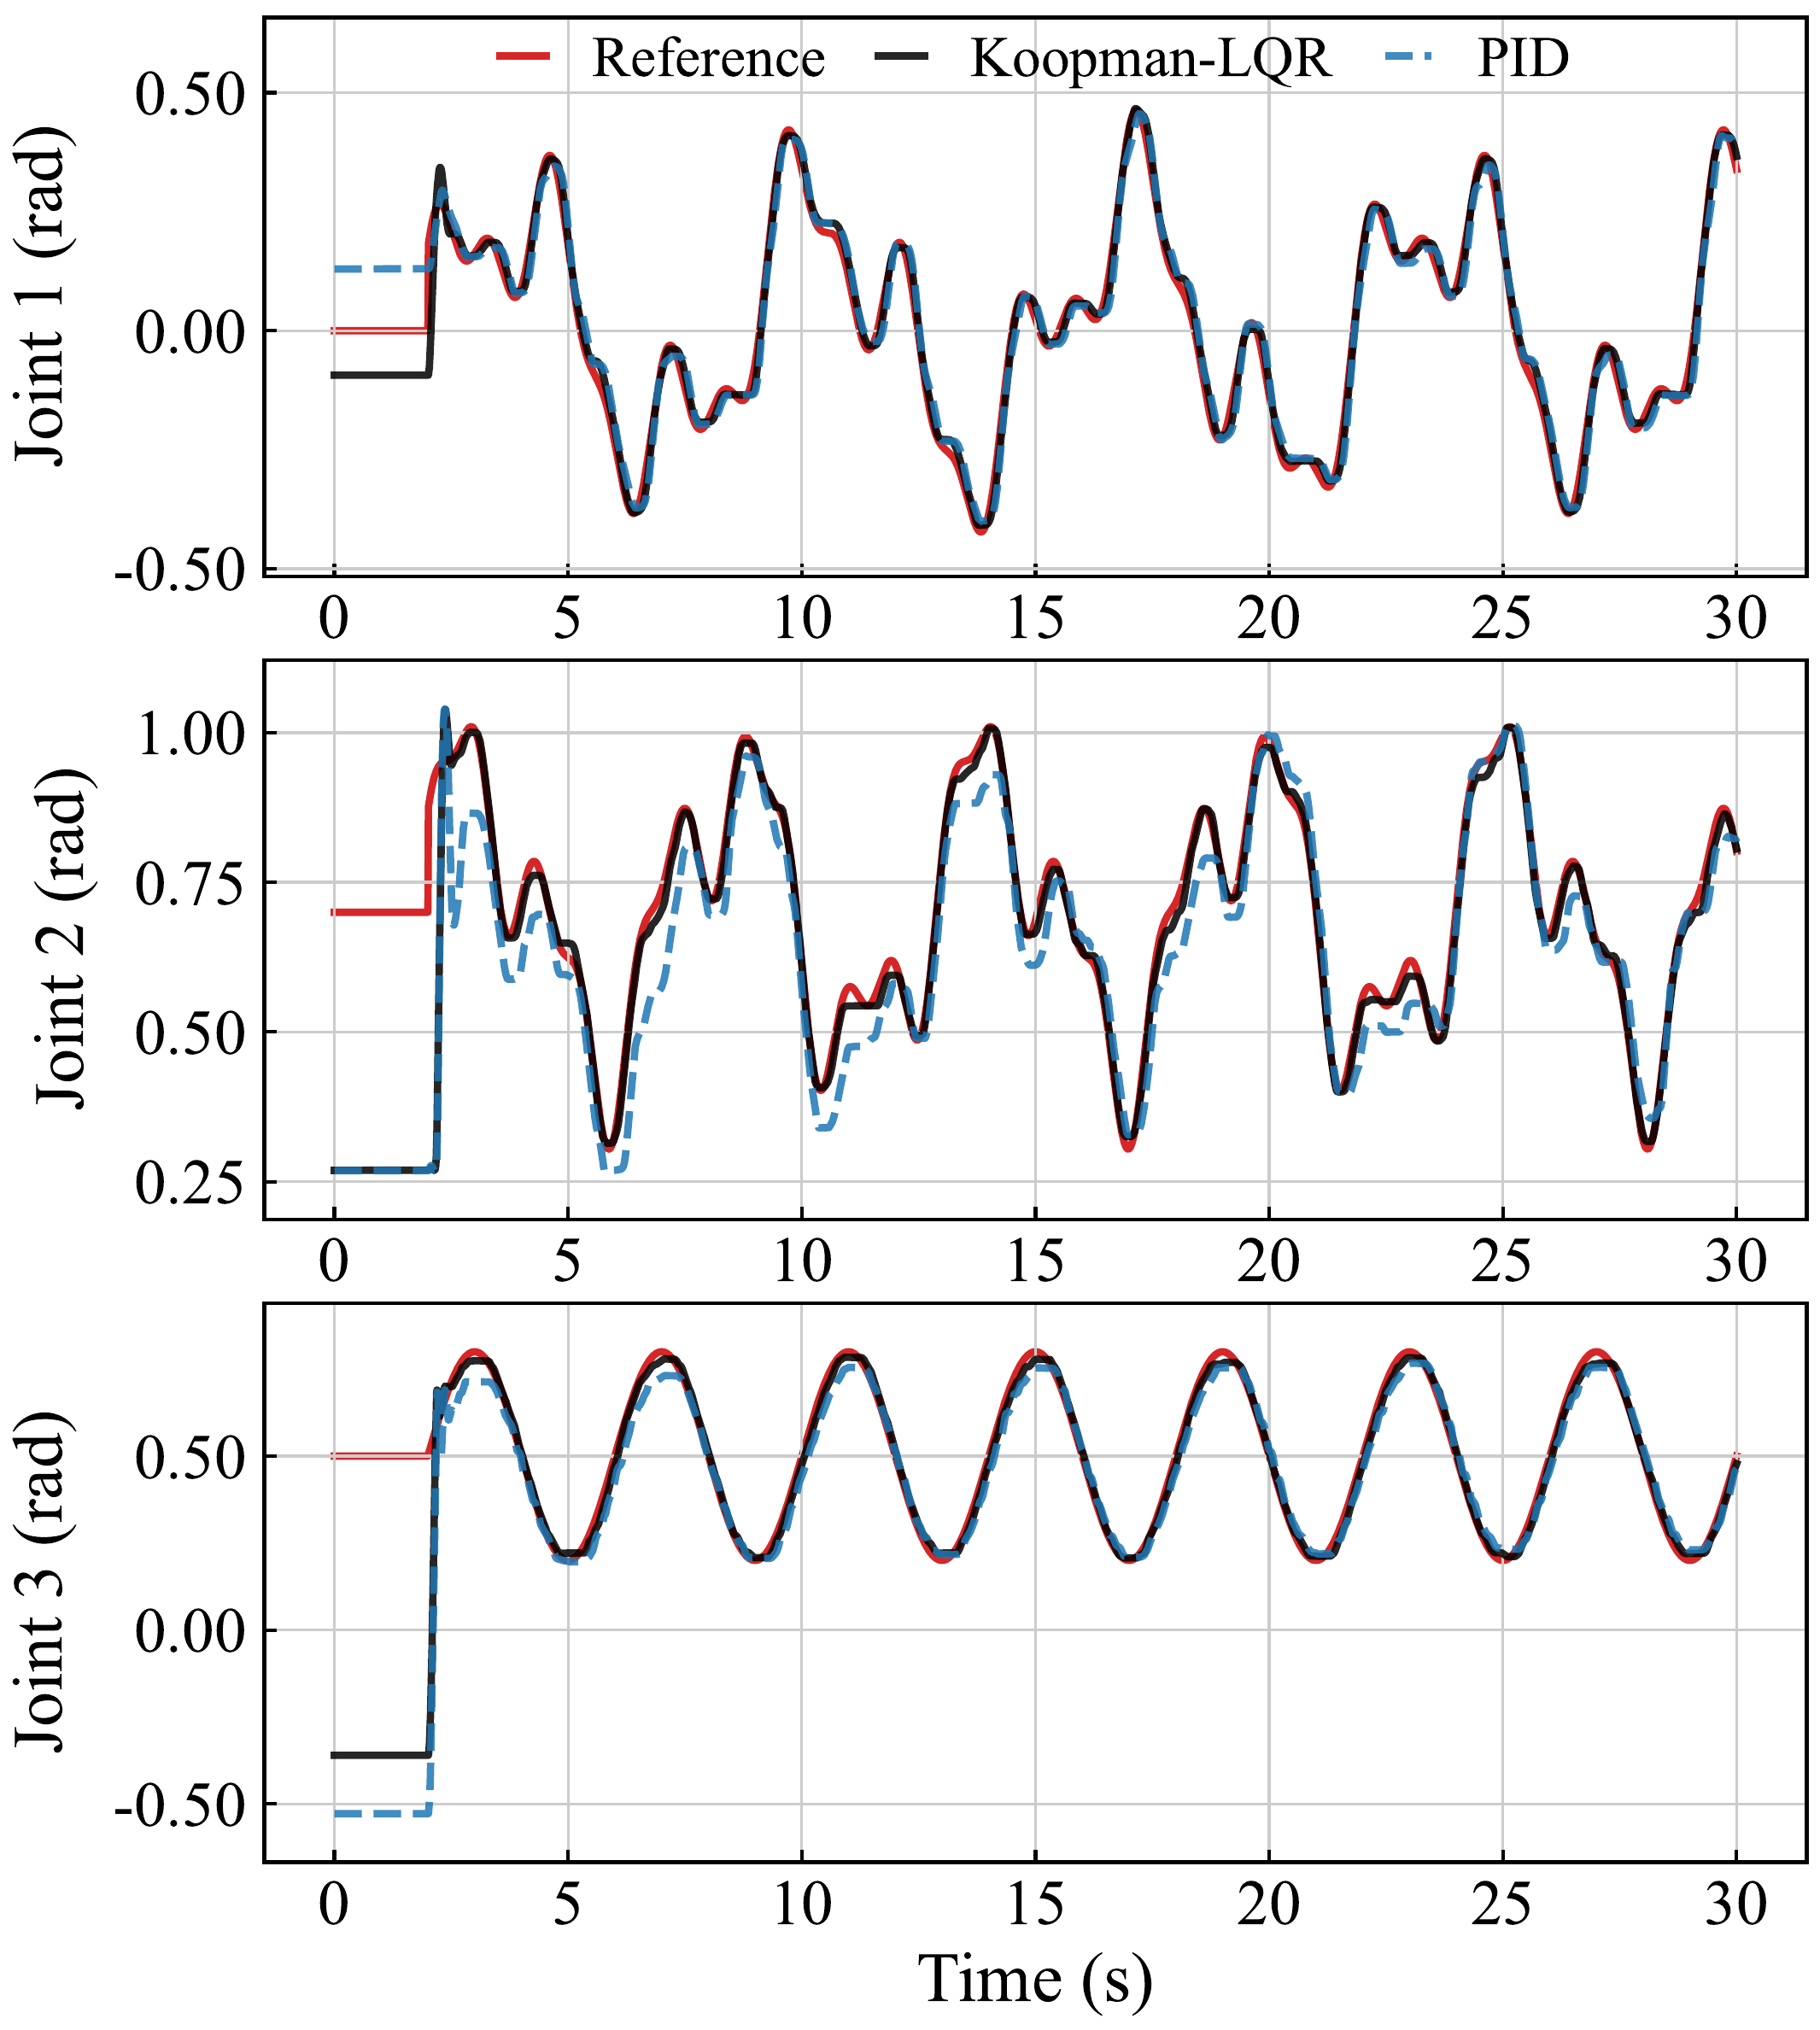
\includegraphics[width=0.4\textwidth]{pictures/control_comparison_irregular.png}
\caption{Comparison of the irregular trajectory tracking performance of the Koopman-LQR and the PID Controllers.}
\label{fig:control_comparison_irregular}
\end{figure}

Table~\ref{tab:control_metrics} summarizes the quantitative tracking results. Koopman-LQR reduces the RMSE$^{\ref{fn:track_metrics}}$/MAE by 42.4\%/66.4\% for sinusoidal tracking and by 9.1\%/38.1\% for irregular tracking, confirming its advantage over PID.

\begin{table}[htbp]
\centering
\caption{Trajectory Tracking Performance}
\label{tab:control_metrics}
\small
\setlength{\tabcolsep}{4pt}
\begin{tabular}{llcc}
\toprule
Type & Controller & RMSE & MAE \\
 &  & (rad) & (rad) \\
\midrule
\multirow{2}{*}{Sinusoidal}
    & Koopman-LQR & \textbf{0.0370} & \textbf{0.0148} \\
    & PID & 0.0642 & 0.0442 \\
\midrule
\multirow{2}{*}{Irregular}
    & Koopman-LQR & \textbf{0.2992} & \textbf{0.0722} \\
    & PID & 0.3293 & 0.1166 \\
\bottomrule
\end{tabular}
\end{table}

\footnotetext[2]{\label{fn:track_metrics}\raggedright
$\mathrm{RMSE}=\sqrt{\frac{1}{3T}\sum_{i=1}^{3}\sum_{k=1}^{T}
(q_i(k)-q_i^{\mathrm{ref}}(k))^2}$, and
$\mathrm{MAE}=\frac{1}{3T}\sum_{i=1}^{3}\sum_{k=1}^{T}
|q_i(k)-q_i^{\mathrm{ref}}(k)|$.}

% ---------------------------------------------------------
\subsection{Robustness Validation Experiments}
\label{subsec:robustness_test}
% ---------------------------------------------------------

Robustness was evaluated using the sinusoidal tracking task with the same controller parameters. During the 30~s experiment, an operator manually disturbed the robot by briefly pushing and pulling the links associated with the three joints, thereby introducing unknown bounded joint torques. As shown in Fig.~\ref{fig:robustness_test}, the joint trajectories exhibit temporary deviations from the references during the disturbances, but recover smoothly after the disturbances are removed and remain bounded throughout the experiment.

\begin{figure}[htbp]
\centering
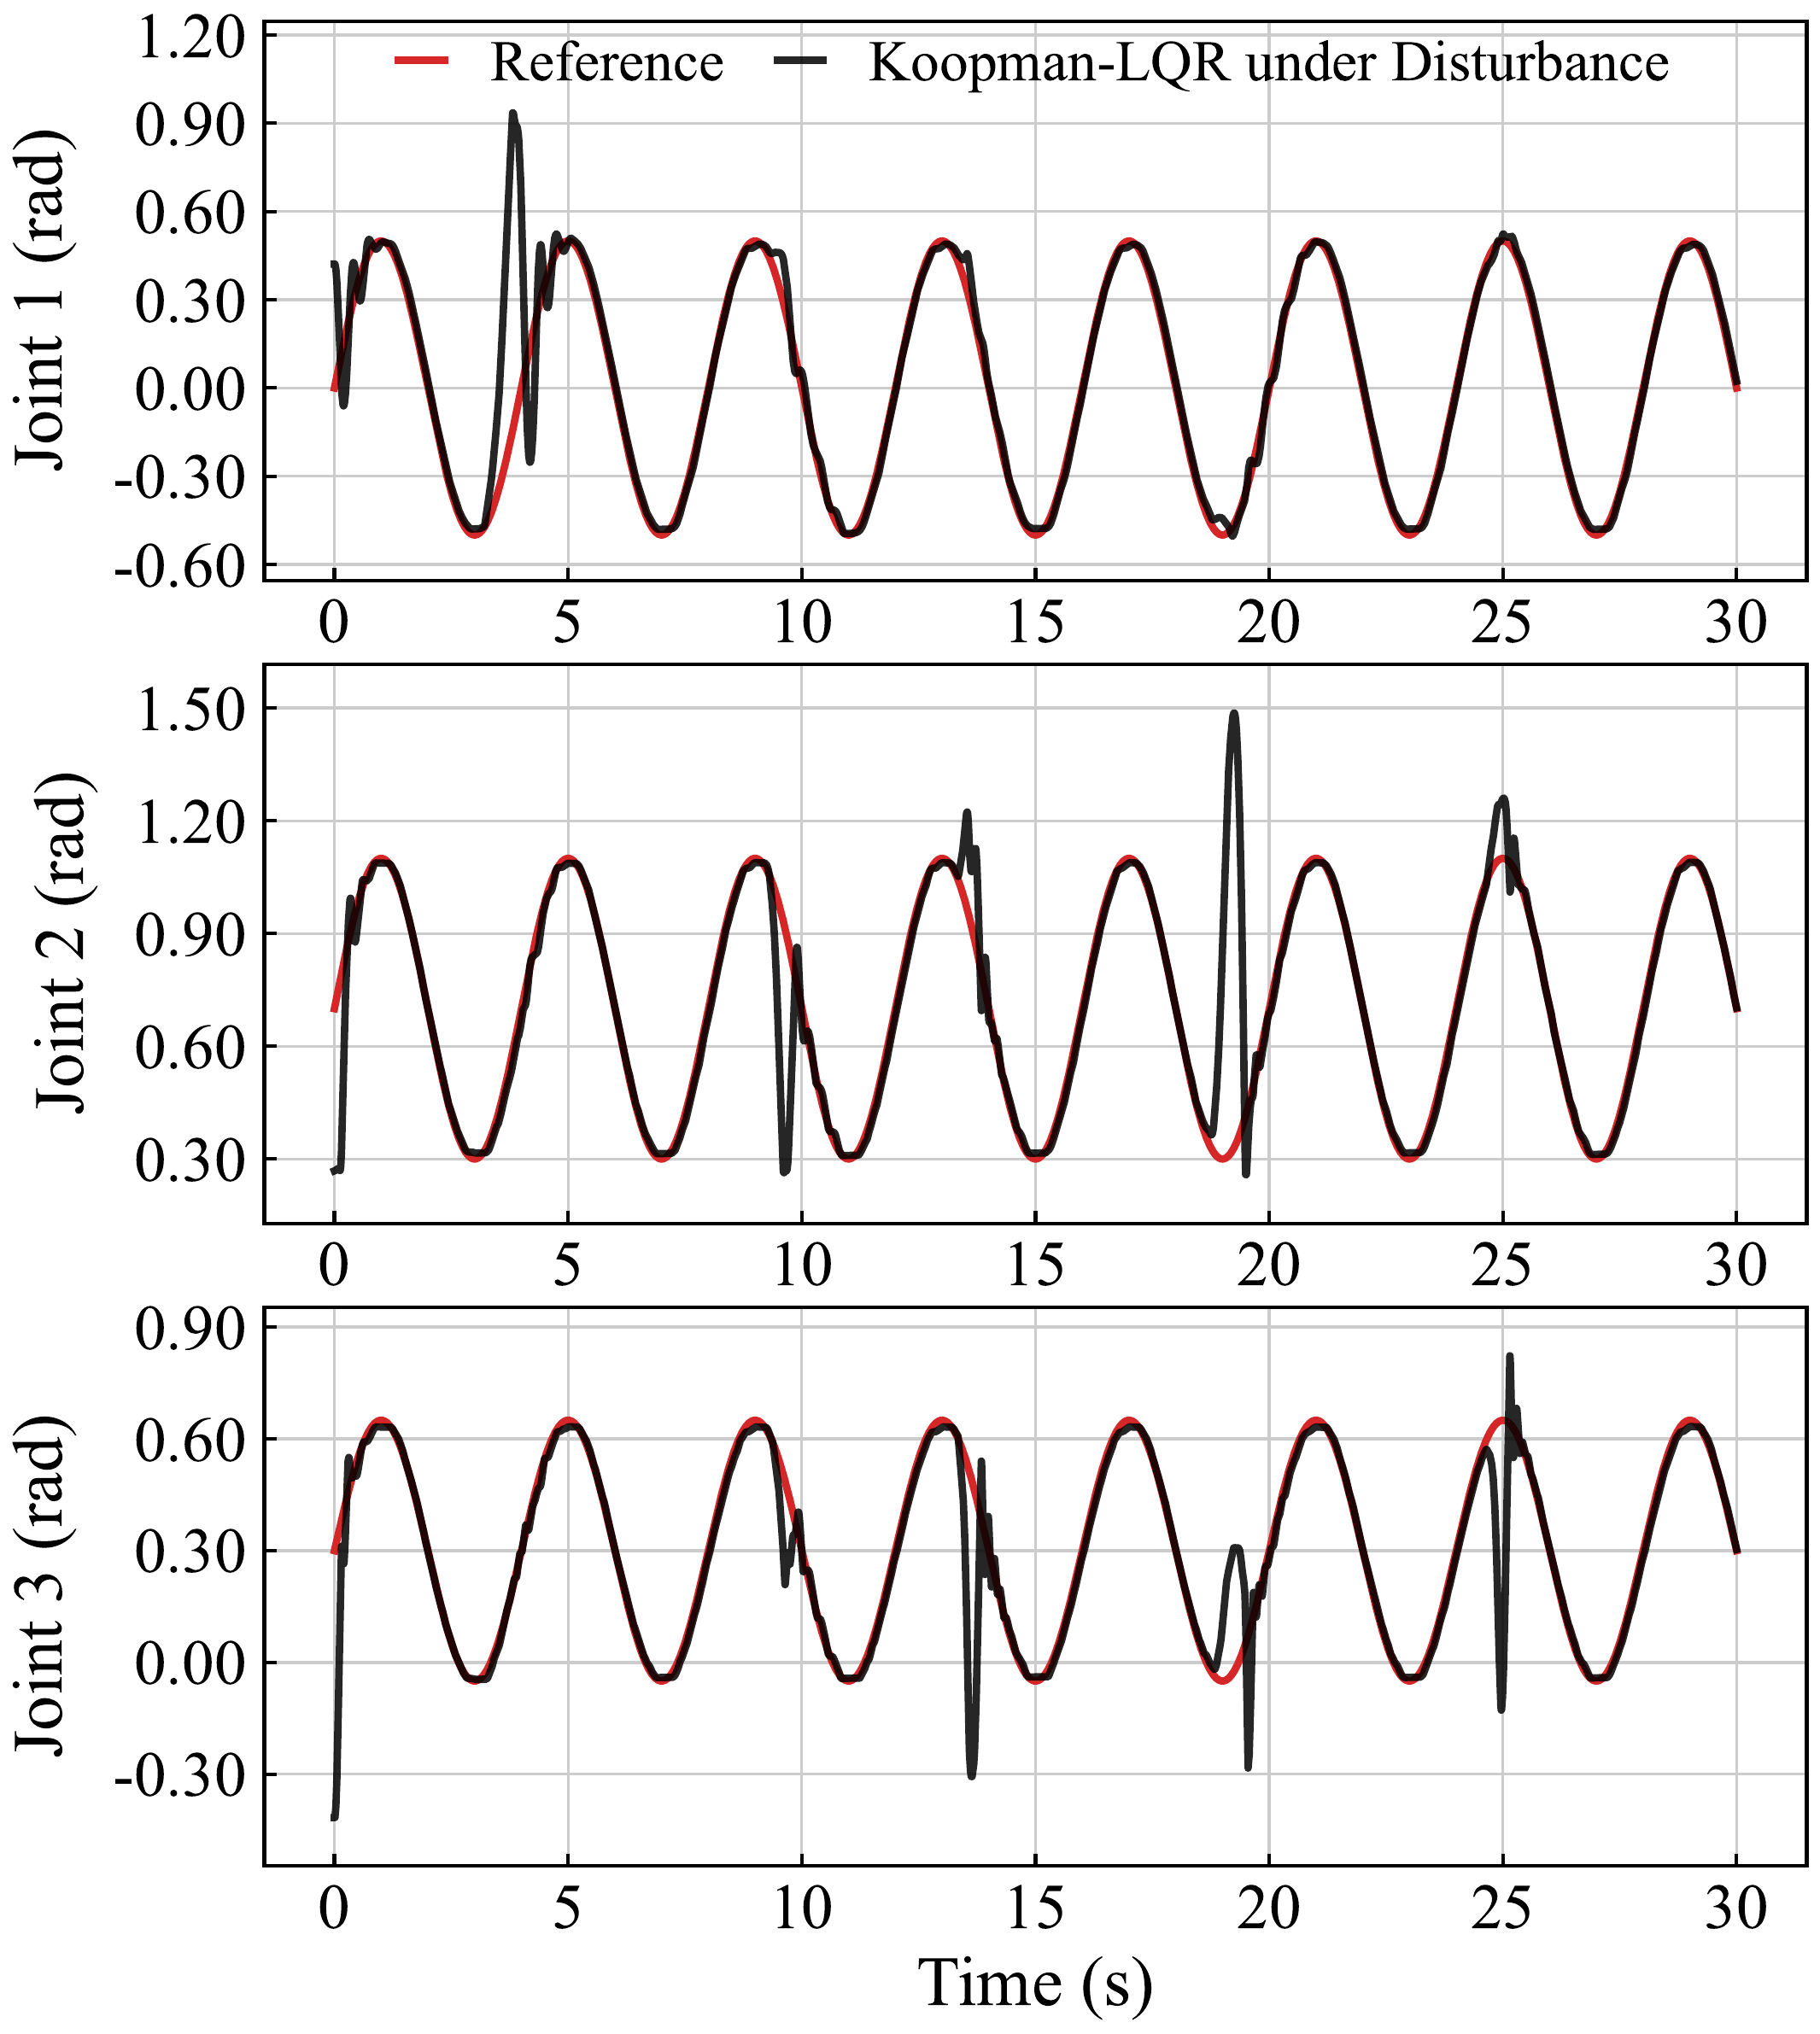
\includegraphics[width=0.4\textwidth]{pictures/robustness_test.png}
\caption{Robustness test under disturbances.}
\label{fig:robustness_test}
\end{figure}





% =========================================================
\section{Conclusion}
\label{sec:conclusion}
% =========================================================

In this paper, we have presented a Koopman representation learning framework with a learnable feature selection matrix to address the tradeoff among modeling accuracy, computational efficiency, and interpretability in dictionary design for EDMD. By constructing an overcomplete physics-informed candidate function library and learning compact feature combinations through an optimizable selection matrix, the proposed method achieves accurate and interpretable Koopman modeling for robotic systems. Based on the learned model, a feedforward--feedback Koopman-LQR controller has been developed, and the ultimate boundedness of the closed-loop tracking error has been established under bounded disturbances. Experimental results on a three-degree-of-freedom robotic arm demonstrate improved prediction accuracy, trajectory tracking performance, and robustness against external disturbances. Future work will consider extending the proposed framework to online learning settings and incorporating model predictive control to explicitly account for state and input constraints.




% ================== References ==================
\bibliographystyle{IEEEtran}
\bibliography{references}


\end{document}
